
% !TEX encoding = UTF-8 Unicode
% !program = pdflatex

\documentclass[11pt,a4paper,bibliography=totoc,listof=totocnumbered]{article}

\usepackage[a4paper,top=30mm,right=20mm,bottom=25mm,left=20mm,head=35mm,foot=15mm]{geometry}
\usepackage[T1]{fontenc}
\usepackage{textcomp}
\usepackage{listings}
\usepackage{fancyhdr}
\usepackage[parfill]{parskip}
\usepackage{algorithm}
\usepackage[noend]{algpseudocode}
\usepackage{amsmath,amssymb}
\usepackage{mathtools}
\usepackage{color}
\usepackage[utf8]{inputenc} % Needed for the Umlaut in our title
\usepackage{pdfpages}
\usepackage{tikz}
\usepackage[acronym]{glossaries}
\usepackage[]{listofsymbols}
\usepackage[style=ieee,sorting=none,backend=biber]{biblatex}
\usepackage{wrapfig}

\addbibresource{citations.bib}

\makeglossaries
\newacronym{ner}{NER}{Named Entity Recognition}
\newacronym{cnn}{CNN}{Convolutional neural network}
\newacronym{iot}{IoT}{Internet of Things}
\newacronym{vsm}{VSM}{Vector space model}

\newglossaryentry{vectoriser}
{
    name=Vectoriser,
    description={A vectoriser transform a text into a numeric vector.}
}
\newglossaryentry{clustering}
{
    name=Clustering,
    description={The task of grouping a set of objects based on their similarity.}
}
\newglossaryentry{docker}
{
    name=Docker,
    description={A tool to package the application with all its dependencies as a single deployable unit and run it on independently from the underlying host.}
}
\newglossaryentry{dockerized}
{
    name=Dockerized,
    description={An application environment running as a single or a collection of docker containers.}
}
\newglossaryentry{api}
{
    name=API,
    description={An application programming interface allowing access to data or features of an application.}
}
\newglossaryentry{stop_word}
{
    name=Stop word,
    description={A term that is overall so frequently used, that it is ignored in natural language processing.}
}

\usetikzlibrary{decorations.pathreplacing}
\usetikzlibrary{positioning}
\lstset{upquote=true}
\lstset{basicstyle=\ttfamily}

\definecolor{codegreen}{rgb}{0,0.6,0}
\definecolor{codegray}{rgb}{0.5,0.5,0.5}
\definecolor{codepurple}{rgb}{0.58,0,0.82}
\definecolor{backcolour}{rgb}{0.95,0.95,0.92}

\lstdefinestyle{mystyle}{
    backgroundcolor=\color{backcolour},   
    commentstyle=\color{codegreen},
    keywordstyle=\color{magenta},
    numberstyle=\tiny\color{codegray},
    stringstyle=\color{codepurple},
    basicstyle=\footnotesize,
    breakatwhitespace=false,         
    breaklines=true,                 
    captionpos=b,                    
    keepspaces=true,                 
    numbers=left,                    
    numbersep=5pt,                  
    showspaces=false,                
    showstringspaces=false,
    showtabs=false,                  
    tabsize=2
}
 
\lstset{style=mystyle}

% language
\usepackage[english]{babel}

% images
\usepackage[font=small,skip=6pt]{caption}
\usepackage{float,graphicx,grffile,wrapfig}
\graphicspath{ {images/} }

% variable definitions
\providecommand{\documenttitle}{Dynamic Event Detection in Data Streams}
\providecommand{\documentauthors}{
  Daniel Milenkovic,
  David Pacassi Torrico
}

\pagestyle{fancy}
\fancyhf{}
\lhead{\documenttitle}
\rhead{\nouppercase{\leftmark}}
\rfoot{Page \thepage}

\begin{document}

\includepdf{templates/cover.pdf}
\includepdf{templates/declaration_of_originality.pdf}

% Der Umfang des Abstracts sollte nicht mehr als eine A4-Seite sein
% (nach DIN / ISO / ANSI beschränkt sich ein Abstract auf ca. 250 Wörter, also eine halbe A4-Seite).

\section*{Abstract}

% Einleitung: definiert die Problematik und begründet die Relevanz der Arbeit.

While searching for events in data streams, the definition of an event might change over time and can therefore not be defined statically depending on one use case. Furthermore, the dynamic behaviour of data streams themselves might change the definition of an event over time.

% Solution
This thesis focuses on developing and evaluating a methodology based on online clustering, where events can be considered either as changes in clusters over time or as the creation of new clusters. The methodology will be applied in the domain of text mining, with data streams consisting of incoming news articles. This allows news articles to be clustered based on their similarity, as similar news articles are considered to be about the same news story. In addition, the evaluation of the clustering quality is measured with a custom scoring function.

% Summary of results
The first part of this work is in determining a suitable data set, which will be the subject of the clustering and at the same time provide the ground truth for evaluating the results. The evaluation focuses on HDBSCAN as the clustering method and compares it with \textit{k}-means, where HDBSCAN is both faster and more accurate. Moreover, different text preprocessing methods and vector space models are evaluated, with text lemmatisation and tf-idf providing the most promising results. Once applied into an simulated online setting, inaccuracies in the overall clustering have a larger impact on event detection. This results in a significant error rate in the detection of new events, while the detection in changes of existing events shows better results. Overall the error rate in event detection is considered to be too high for real world applications and a possible continuation of this work could be improving the clustering to decrease the error rate in detecting events.



\section*{Preface}
\label{sec:preface}

The following bachelor thesis \textit{Dynamic Event Detection in Data Streams} was written
as part of our computer science studies at the ZHAW Zurich University of Applied Sciences.

After our lectures on artificial intelligence, we realized that we wanted to deepen our knowledge in this area.
This thesis was the perfect opportunity to increase our expertise on topics such as natural language processing
and cluster analysis.

Special thanks go to our two supervisors, Dr. Andreas Weiler and Prof. Dr. Kurt Stockinger,
for their ongoing and effective support during the writing of this thesis.

We would also like to thank our two lecturers Prof. Dr. Thilo Stadelmann
and Prof. Dr. Mark Cieliebak for their lectures on artificial intelligence.

At last but not least, we would like to thank our fellow students
and the entire ZHAW staff for our great time at ZHAW.

Daniel Milenkovic and David Pacassi Torrico

\include{0_table_of_contents}
\section{Introduction}
\label{sec:introduction}

\subsection{Problem Formulation}
\label{subsec:problem_formulation}
% Wie kann in einem Datenstrom Ereignisse erkannt werden?

% Bei der Suche nach neuen Ereignissen in Datenströmen, kommt es immer zum Problem was ein Ereignis genau ist. Wenn diese erste Frage geklärt ist kommt es aber zu weiteren Fragestellungen. Meistens reicht es nicht ein Ereignis statisch zu definieren, sondern die Definition entwickelt sich dynamisch über die Zeit. Die meisten Verfahren zu Ereigniserkennung werden aber bei Systemstart statisch eingestellt. Weiterhin muss man stets die Dynamik des Streams beachten, da es sonst du Blockaden und Überlauf im System kommen kann.

% Ziel dieser Arbeit ist es eine Methodik zu entwickeln wie die genannten Aspekte auf geeigneten Datenströmen umgesetzt werden können.


How can events be recognized in a data stream?
While searching for events in a data stream, the definition of an event is not always clear.
Providing static definitions, as most approaches do,
does not suffice for dynamic data streams, which change over time.
Additionally, the behaviour of the data stream is an important factor in itself,
since blockages of overflows in the system have to be prevented.

An example for a dynamic data stream can be found in a stream of news articles, which are published in irregular time intervals and different quantities over time. Thus detecting events based on an incoming stream of news articles is a challenging task.

The goal is to develop and evaluate a methodology to detect events in a dynamic stream of news articles.

\subsection{Motivation}
\label{subsec:motivation}
Today's environment is rapidly changing.
With more devices being digitalized and connected to the internet,
we are starting to have incredible amounts of data.
Every smartphone, smartwatch and many other \gls{iot} devices start tracking every sensor data they record.

There is and will be no way to process all this data manually.
This is where our work becomes relevant.
We will try to detect events from a data stream, even when new and unknown events arise.

Our solution is based on text data, so any data in text form should be applicable.
With technologies such as speech recognition, the data could also initially be acoustic
and converted to text before being entered into our application.

That would open up use cases with smart speakers such as \textit{Amazon Echo} or \textit{Google Assistant}.

% lol stay humble david ;)
% \paragraph{Personal motivation}
% We have a combined experience of 17 years working in the IT sector together,
% for our bachelor thesis we wanted to do something more challenging than
% developing a simple application.

\section{Related Work}

\subsection{Related Work \# 1}
Text based event detection is a diverse field and with increasingly large amounts of available information online a compelling topic for research.
With the popularity of social media a lot of research around event detection has been done on microblogs\cite{microblog_clustering} such as Twitter\cite{twitter_survey}\cite{social_media_survey}.
However this thesis focuses on news articles as the primary data source.
Text based clustering as a technique for event detection has already been explored with different approaches such as using custom methods based on neural networks\cite{text_clustering_topic_detection}
or by using a modified version of DBSCAN to account for its sensitivity for differences in cluster densities\cite{dbscan_martingale}.
Based on the promising results with DBSCAN we want to further explore text clustering using its successor HDBSCAN\cite{McInnes2017} and apply it in an online setting.
Regarding the clustering validation there has already been research into recognising biases of different scoring functions \cite{Wu:2009:ARM:1557019.1557115}
and developing custom scoring functions as a result\cite{gates2017comparing}.

\subsection{Related Work \# 2}
Todo.

\subsection{Related Work \# 3}
Todo.

\section{Theoretical basics}
In order to fully understand our work,
it is important to ensure a few basics in the area of natural language processing (NLP).
In this chapter we'll explain how the most important techniques used in our thesis work.

\subsection{Text preprocessing}
\label{sec:text_preprocessing}

When working with text data, many algorithms and processes will need to distinguish words from another.
In most cases this is done by creating a dictionary of all known words and/or by \textit{vectorizing} text data
in order to make them comparable.
While this works in theory, in reality we deal with a tremendous amount of data.
This results in huge directories or many vectors and does not only take up more disk space
but also text processing (computation and comparison) will take more time to process.

What does that mean?
Let's have a look at the following words:

\begin{itemize}
    \item switzerland
    \item Switzerland
    \item SWITZERLAND
\end{itemize}

Anyone of us will be able to extract the same meaning out of these three words: The country \textit{Switzerland}.
However, for machines the terms are different because they're written differently.
That's why in most cases it makes sense to lowercase all text before processing them.
That way we can ensure that the above words also share the same meaning for a machine and thus reduce the dictionary size.

% TODO: \paragraph{extraction}

Lowercasing text can just be the beginning though.
Depending on the size of a document, it might make sense to not use all text inside a document.
A good example for this would be books.
Vectorising books would take too much computational power and time to process.
In such cases, the text size would have to be reduced.
This could be accomplished by processing a summary of the book instead of the book itself
or by extracting the most relevant words from the whole book.
Later could be done with \textit{Keyterm extraction} or with \textit{Entity extraction}.

% TODO: \paragraph{lemma stemma}
If we're not dealing with books but with articles or papers,
there are also other alternatives to Keyterm and Entity extraction.
Using \textit{Text Stemming} or \textit{Text Lemmatisation} we can simplify terms and group them together to reduce
the dictionary size.
More about this in the sub sections below.

\paragraph{Exceptions}
There are a few use cases where lowercasing a text isn't desired.
For example when trying to detect the writer's sentiment.
Someone who would write a few or all words of a sentence in uppercase might be angrier than someone who doesn't.

\subsubsection{Keyterm extraction}
Todo.

\subsubsection{Named Entity Recognition}
Todo.

\subsubsection{Text Stemming}
Text Stemming is a form of Text Normalization which aims to simplify words
by reducing the inflectional forms of each word into their word stems.
For example, the words \textit{connected}, \textit{connecting}, \textit{connection} share a similar meaning and could
therefor be simplified to the base term \textbf{connect}.

The first paper describing a stemming algorithm was written by Julie Beth Lovins\cite{LovinsStemmer}
as early as in 1968.
In her algorithm she used an ordered list of 294 suffixes to strip them out and then applies one of
29 associated application rules followed by a set of 35 rules to check if the remaining stem has to be
modified furtherly.

Lovins' stemming algorithm was very successful but got mostly replaced by
M.F. Porters stemming algorithm\cite{PorterStemmerAlgorithm} published in 1980.
In his paper, M.F. Porter was able to process his suffix stripping algorithm in 6'370 out of 10'000 words and thereby
reducing the vocabulary size by \textbf{one third}.
The algorithm simply follows 5 steps with replacement and/or removal rules and is therefor very easy and efficient.

M.F. Porter improved his stemming algorithm even further by publishing the Porter2 stemming algorithm\cite{SnowballStemmerAlgorithm} in 2002
which is widely known as the \textit{Snowball stemming algorithm}.

There are even more stemming algoriths, very well known are the Lancester stemming algorithm\cite{LancesterStemmer}
and the WordNet stemming algorithm\cite{WordNetStemmer}.
Since M.F. Porter's snowball stemming algorithm is the most widely used one, we decided to go with his algorithm.

\subsubsection{Text Lemmatisation}
Similar to \textit{Text Stemming}, Text Lemmatisation has the same goal to group together the inflected forms of a word
but follows a different approach to do so.
Instead of processing terms with fixed steps and defined rules,
Text Lemmatisation normally includes a dictionary lookup for the words
and also takes in consideration to which part of a sentence a term belongs to.
This results in more accurate root terms but also asks for more computational power than Text Stemming.
See following table for a comparison:

\begin{table}[h]
    \centering
    \begin{tabular}{|l|l|r|r|}
    \hline
    \textbf{\#} & \textbf{Original word} & \textbf{Stemmed} & \textbf{Lemmatised} \\ \hline
    1 & written & written & write \\ \hline
    2 & greatest & greatest & great \\ \hline
    3 & best & best & best \\ \hline
    4 & fastest & fastest & fastest \\ \hline
    5 & highest & highest & high \\ \hline
    6 & compute & comput & compute \\ \hline
    7 & computer & comput & computer \\ \hline
    8 & computed & comput & compute \\ \hline
    9 & computing & comput & compute \\ \hline
    10 & studies & studi & study \\ \hline
    11 & studying & studi & study \\ \hline
    12 & university & univers & university \\ \hline
    13 & universities & univers & university \\ \hline
    14 & universe & univers & universe \\ \hline
    15 & universal & univers & universal \\ \hline
    \end{tabular}
    \caption{Comparison of Text Stemming and Text Lemmatisation.}
    \label{tab:comparison_stemming_lemmatisation}
\end{table}

% TODO: Talk about time.

\subsection{Data Representation}
Todo.

\subsubsection{Word Frequency}
Todo.

\subsubsection{tf-idf}
Todo.

\subsection{Clustering}
Clustering finds similarities in different news articles based on their content and groups them together,
while unrelated news are regarded as noise.
The challenge now arises to find an appropriate clustering method,
which is able to work with data of varying densities and of high dimensionality.

% TODO why hdbscan

\subsubsection{\textit{k}-means clustering}
\textit{k}-means clustering is an iterative clustering method which assigns all data points in a given data set
into k clusters, where k is a predefined number of clusters in the data set.

\paragraph{How does k-means clustering work}
At the very beginning, k-means creates k centroids at random locations.
It then repeats following instructions until reaching convergence:

\begin{itemize}
    \item For each data point: Find the nearest centroid
    \item Assign the data point to the nearest centroid (cluster)
    \item For each cluster: Compute a new cluster centroid with all assigned data points
\end{itemize}

\paragraph{Advantages}
\begin{itemize}
    \item Very simple and easy to understand algorithm
\end{itemize}

\paragraph{Disadvantages}
\begin{itemize}
    \item Initial (random) centroids have a strong impact on the results
    \item The number of clusters (k) has to be known beforehand
    \item Unable to handle noise (all data points will be assigned to a cluster)
\end{itemize}

\subsubsection{DBSCAN}
DBSCAN stands for \textit{Density-Based Spatial Clustering of Applications with Noise}
and is a density based clustering algorithm.

A big advantage of DBSCAN is that it is able to sort data into clusters
of different shapes.

\paragraph{How does DBSCAN work}
DBSCAN requires two parameters in order to work:

\begin{enumerate}
    \item epsilon - The maximum distance between two data points for them to be considered as in the same cluster.
    \item minPoints - The number of data points a neighbourhood has to contain in order to be considered as a cluster.
\end{enumerate}

Having these two parameters defined, DBSCAN will iterate through the data points
and try to assign them to clusters if the provided parameters match.
If a data point can't be assigned to a cluster, it will be marked as noise point.

Data points that belong to a cluster but don't dense themselves are known as \textbf{border points}.
Some border points could theoretically belong to two or more clusters
if the distance from the point to the clusters don't differ.

\paragraph{Advantages}
\begin{itemize}
    \item Does not need to know the number of clusters beforehand.
    \item Is able to find shaped clusters.
    \item Is able to handle noise points.
\end{itemize}

\paragraph{Disadvantages}
\begin{itemize}
    \item DBSCAN is not entirely deterministic.
    \item Defining the right epsilon value can be difficult.
    \item Unable to cluster data sets with large differences in densities.
\end{itemize}

\subsubsection{HDBSCAN}

HDBSCAN is a hierarchical density-based clustering algorithm \cite{McInnes2017}, based on DBSCAN and improves its sensitivity for clusters of varying densities. Therefore defining an epsilon parameter, which acts as a threshold for finding clusters, is no longer necessary. This makes the algorithm more stable and flexible for different applications. 


\paragraph{How HDBSCAN works}


Since HDBSCAN is the focus for this thesis, we want to give a more detailed explanation of its inner workings, than for \textit{k}-means or DBSCAN.

HDBSCAN only requires one parameter to be set beforehand:
\begin{enumerate}
    \item minPoints - The number of data points a neighbourhood has to contain in order to be considered as a cluster.
\end{enumerate}

The algorithm consist of five steps, which are as follows: 

\subparagraph{1. Transforming the space}

At its core HDBSCAN is a single linkage clustering, which are typically rather sensitive to noise. A single noise point between clusters could act a bridge, which would result in both clusters to be seen as one. To reduce this issue, the first step is to increase the distances of lower density points. This is achieved by to comparing the core distances between two points with the original distance to get the the mutual reachability distance. The core distance $core_k(x)$ is defined as the radius of a circle around point $x$, so that $k$ neighbours are contained within this circle. TODO describe example in Figure \ref{fig:hdbscan_1}. 

\begin{figure}[h]
    \centering
    \includegraphics[width=0.5\textwidth]{hdbscan_1}
    \caption{The core distances. TODO give more detailed explanation.}
    \label{fig:hdbscan_1}
\end{figure}

Once the core distances are known, the mutual reachability distance between two points is defined as follows:

\begin{equation*}
    d_{mreach}(a, b) = max\{core_k(a), core_k(b), d(a, b)\}
\end{equation*}

where $d(a, b)$ is the original distance between $a$ and $b$. Therefore if two points are close together, but the density around one point is rather low, the core distance will be greater than the original distance and thus the two points appear to be less close together when considering the mutual reachability distance.

\subparagraph{2. Build the minimum spanning tree}

Based on the mutual reachability distances, the next step is to find points close  to each other. This is done by creating a minimum spanning tree, where edges are weighted according to the mutual reachability distance and a point is represented by a vertex. The minimum spanning tree is created one edge at a time, always choosing the lowest distance to a vertex not yet in the tree. This is done until each vertex is connected, which results in the minimal set of edges, such that dropping any edge will cause the disconnect of one or more vertices from the tree.

\subparagraph{3. Build the cluster hierarchy}

Once the minimum spanning tree is complete, it is converted into a hierarchy of connected clusters, by sorting edges of the tree by distance and iterate through, creating a new merged cluster for each edge. The dendogram in Figure \ref{fig:hdbscan_2} shows a possible cluster hierarchy. %TODO rewrite this paragraph. 

\begin{figure}[h]
    \centering
    \includegraphics[width=0.5\textwidth]{hdbscan_2}
    \caption{The cluster hierarchy shown as a dendogram}
    \label{fig:hdbscan_2}
\end{figure}

At this stage we have to flatten the hierarchy to get the final clusters, which provide the best representation of the current data set. DBSCAN simply cuts through the hierarchy using a fixed parameter, usually called epsilon, to get the final clusters. This approach does not work well with clusters of varying densities and the epsilon parameter itself is unintuitive, requiring further exploration to find optimal values. This is were HDBSCAN improves upon DBSCAN, by taking additional steps for finding relevant clusters.

\subparagraph{4. Condense the cluster tree}

\begin{figure}[h]
    \centering
    \includegraphics[width=0.5\textwidth]{hdbscan_3}
    \caption{Condensed cluster hierarchy}
    \label{fig:hdbscan_3}
\end{figure}

The fourth step consists of condensing the previously built cluster hierarchy into a smaller tree. The process starts at the top where all vertices still belong to the same cluster. Iterating through the hierarchy, for each split the two resulting clusters are compared against a predefined minimum cluster size. If the size of a cluster is below the minimum, its points will be discarded, while the other cluster remains in the parent cluster. If both cluster sizes are above or equal the minimum, the clusters are considered as true clusters. This is repeated until no more splits can be made. 


\subparagraph{5. Extract the clusters}

The extraction of the final clusters from the condensed tree is based on the stability per cluster and once it is selected, none of its subclusters can be chosen. The stability is based on the persistence of a cluster, which is measured by $\lambda = \frac{1}{distance}$. The stability for a cluster $C$ is defined as

\begin{equation}
\sum_{p \in \text{C}}^{|C|} ({\lambda}_{p} - {\lambda}_{birth})
\end{equation}

 where ${\lambda}_{p}$ describes when point $p$ fell out of the cluster and $ {\lambda}_{birth}$ describes when the cluster was created. Now calculating the stability for each cluster starts at the leaf nodes and ends when the root is reached. A cluster is selected if its stability is larger the sum of stabilities of its children. If the sum child stabilities is larger than that of its parent, the parent stability will be set to the value of the sum of its children, but no selection will be done. Based on this approach the final clusters will be selected, with regards to varying densities and noise.
\section{Design and Implementation}
\label{sec:4_design_and_implementation}

The methodology consist of three parts, where each part builds upon the results from the previous one.
Initially the test data is created, which will be used for all evaluations.
Secondly we evaluate HDBSCAN and determine the optimal settings for our use case.
The final part applies the results obtained from the previous evaluation in an online setting.

\subsection{Dataflow}
\label{subsec:4_dataflow}

The dataflow, see \figref{fig:dataflow}, starts with receiving new news articles every hour.
The articles content will then be preprocessed (see \subsecref{subsec:3_text_preprocessing})
and vectorized.
With the computed vectors, the articles will then be clustered to existing or new news stories.
The cluster changes represent our detected events.

\begin{figure}[!htb]
    \centering
    
\begin{tikzpicture}[
            squarednode/.style={rectangle, align=center, draw=black!60, very thick, minimum size=5mm},
        ]

        % Nodes.
        \node[squarednode] (incoming_data)                               {Incoming\\news articles};
        \node[squarednode] (preprocessing)   [right=of incoming_data]    {Text\\preprocessing};
        \node[squarednode] (vectorization)   [right=of preprocessing]    {Vectorization};
        \node[squarednode] (clustering)      [right=of vectorization]    {Clustering};
        \node[squarednode] (event_detection) [right=of clustering]       {Event\\detection};

        % Lines.
        \draw[->] (incoming_data.east) -- (preprocessing.west);
        \draw[->] (preprocessing.east) -- (vectorization.west);
        \draw[->] (vectorization.east) -- (clustering.west);
        \draw[->] (clustering.east) -- (event_detection.west);
    \end{tikzpicture}

    \caption{Dataflow}
    \label{fig:dataflow}
\end{figure}

\subsection{Data Set}
\label{subsec:4a_data_set}

Before any clustering method can be implemented or evaluated,
it is important to rely on the right data set for training and evaluation.

\subsubsection{Data Set Candidates}
\label{subsubsec:4a_data_set_candidates}

As our goal is to detect events in data streams, we've evaluated different data sets and
their possibilities to extract events from their data themselves.

\begin{table}[h]
    \centering
    \begin{tabular}{|l|r|l|}
    \hline
    \textbf{Data set} & \textbf{Number of rows} & \textbf{Description} \\ \hline
    GDELT 2.0 & 575'000'000+ & Print and web news from around the world. \\ \hline
    ChallengeNetwork & 4'449'294 & Network packages including anomalies. \\ \hline
    One Million Posts Corpus & 1'011'773 & User comments to news articles. \\ \hline
    Online Retail Data Set & 541'909 & Customer retail purchases of one year. \\ \hline
    News Aggregator Dataset & 422'937 & Clustered news articles. \\ \hline
    Dodgers Loop Sensor Data Set & 50'400 & Number of cars driven through a ramp. \\ \hline
    10k German News Articles & 10'273 & German news articles. \\ \hline
    \end{tabular}
    \caption{Evaluated data set candidates ordered by data set size.}
    \label{tab:data_set_candidates}
\end{table}

We could extract events from all data sets mentioned in Table \ref{tab:data_set_candidates}.\\
The extracted events could be as follows:

\begin{itemize}
    \item Network packages
        \begin{itemize}
            \item Cyber attacks depending on suspicious packets.
        \end{itemize}
    \item User comments
        \begin{itemize}
            \item Change of public opinion during time.
        \end{itemize}
    \item Retail purchases
        \begin{itemize}
            \item Change of purchasing behavior based on product choices.
        \end{itemize}
    \item Traffic
        \begin{itemize}
            \item Traffic changes due to baseball games.
        \end{itemize}
    \item News articles
        \begin{itemize}
            \item Development of a certain news story.
        \end{itemize}
\end{itemize}

However, from above data sets only two contained prelabeled events:

\begin{enumerate}
    \item Dodgers Loop Sensor Data Set
        \begin{itemize}
            \item 81 labeled events. % Todo: x events in y clusters
        \end{itemize}
    \item News Aggregator Dataset
        \begin{itemize}
            \item 422'937 labeled events. % Todo: x events in y clusters
        \end{itemize}
\end{enumerate}

As we didn't want to lose too much time in manually clustering data, we've decided to go with one of these two.
Regarding our two options, our choice was simple:\\
We went for the \textbf{The News Aggregator Dataset} since it not only provided more data,
but our work built on the news articles use case could later be continued with real live data.
The \textbf{GDELT 2.0} data set for example, provides around 1'000 to 2'000 new news articles every 15 minutes.

\subsubsection{Data Retrieval}
\label{subsubsec:4a_data_retrieval}

Unfortunately the data set did not contain the news articles themselves but rather only the URL's to the news articles.
This was done so due to copyright restrictions on the content.
Fortunately there are web scraping tools designed to retrieve the content from news articles specifically.
We decided to use Newspaper3k\cite{newspaper3k},
a Python3 library that allows us to retrieve the text from news articles easily.

The library only requires an URL to download and extract the news article from a website, see following example:

% Todo: Hyphen gets converted inside "lstlisting". Copy & paste the URL from the PDF into a browser -> it won't work.
\begin{lstlisting}[language=Python, caption=Retrieve the news article from an URL., label={lst:newspaper3k_code}]
    from newspaper import Article

    url = 'http://fox13now.com/2013/12/30/new-year-new-laws-obamacare-pot-guns-and-drones/'
    article = Article(url)
    article.download()
    article.text # Contains the article's text.
\end{lstlisting}

All we had to do now is to run this code for all news articles.
To speed this process up, we've loaded the data set into a database and run 8 concurrent processes which
retrieved the news articles content from the web in different batches.

\subsubsection{Data Cleansing}
\label{subsubsec:4a_data_cleansing}

The data set contains news articles collected from March 10th to August 10th of 2014.
Five years later, many resources are not online anymore or are not accessible from Europe due to GDPR.
We've used following SQL query to filter out news articles that were most likely corrupt:

\begin{lstlisting}[language=SQL, caption=Retrieve valid news articles., label={lst:valid_news_articles_sql}]
    SELECT *
    FROM news_article
    WHERE
        newspaper_text IS NOT NULL
        AND TRIM(COALESCE(newspaper_text, '')) != ''
        AND hostname NOT IN ('newsledge.com', 'www.newsledge.com')
        AND newspaper_text NOT LIKE '%GDPR%'
        AND newspaper_text NOT LIKE '%javascript%'
        AND newspaper_text NOT LIKE '%404%'
        AND newspaper_text NOT LIKE '%cookie%'
        AND newspaper_keywords NOT LIKE '%GDPR%'
        AND newspaper_keywords NOT LIKE '%javascript%'
        AND newspaper_keywords NOT LIKE '%404%'
        AND newspaper_keywords NOT LIKE '%cookie%'
        AND title_keywords_intersection = 1
\end{lstlisting}

% Todo: Continue cleansing text.

% Todo: The first important step is to create a test data set to run the evaluations with and verify them.
% Todo: explain the source and structrue

% raw text
% with entity extraction
% word embeddings?
% Tfidf

\subsection{Clustering Evaluation}
\label{subsec:4b_clustering_evaluation}

\subsubsection{Design}
\label{subsubsec:4b_design}

The clustering evaluation will focus on HDBSCAN as the main clustering method. 
The properties of HDBSCAN are a good fit for our use case of clustering news articles in an online setting.
It is able to work with clusters of varying densities, 
does not require to know the number of clusters in advance 
and is efficient with a time complexity of $O(nlog(n))$.
The density requirement is based on our test data, which contains clusters with sizes ranging from 2 to over 400. 
In addition, we do not know the number of clusters in the data stream and therefore can not provide an approximation
beforehand. This already disqualifies a wide range of clustering methods such as \textit{k}-means. 
Another feature of HDBSCAN is its ability to discard samples as noise. 
This can be a useful feature once applied to an online setting, 
since noisy data is to be expected in a data stream from external sources. 

The goal of the clustering evaluation is to find the optimal parameters and preprocessing methods
for running HDBSCAN on our test data and to measure the overall performance.
Therefore the clustering evaluation is designed to run HDBSCAN using a combination of different text processing methods, vector space models and parameters.
\textit{k}-means is used to provide a benchmark for the HDBSCAN evaluation.
Once a clustering has been performed,
the result is measured based on the ground truth and stored in a database for later analysis.

An important consideration is the variety of samples to use for a single clustering.
Using one set of samples might bias the score against this specific set of samples
and some methods might perform better or worse depending on the samples.
To introduce variability, while still retaining repeatability, an evaluation run will be repeated multiple times.
Each repetition will load a new set of samples, iterating linearly through the data set.
For example if we define the number of repetitions as 2 with a sample size of 1000,
the evaluation will be done on the first 1000 samples with all possible settings
and the second run will load the next 1000 samples, thus containing samples with indices ranging from 1001 to 2000.
The reason we do not load random sets of samples is repeatability.
If we make any changes in the implementation or the scoring function,
we want to be able to compare the new results with the previous ones in a deterministic manner.

Furthermore, news articles are loaded based on their stories. 
Thus an evaluation done with 30 stories, will actually load all news articles belonging to these stories.
This is done to prevent stories from being cut off, resulting in potential noise.

\subsubsection{Scoring Function}
\label{subsubsec:4b_scoring_function}

The scoring function is essential for evaluating the result of a clustering method.
The score should reflect the quality of the individual clusters and of the clustering as a whole.
The number of existing measures for clustering is vast and can be split into three main categories.
Internal measures determine the score based on criteria derived from the data itself,
 external measures depend on criteria non-existent in the data itself such as class labels
 and relative measures compare different clusterings with each other.
Since the ground truth is known in our test data, we are going to apply an external measure.

Initially we used \gls{nmi} as our primary scoring function.
\gls{nmi} is an entropy-based measure and tries to quantify the amount of shared information between predicted clusters and the ground truth.
The score proved to work well for our initial evaluations, but upon closer inspection certain anomalies were found.
An example is given in \tabref{tab:nmi_kmeans_example}, where \textit{k}-means achieved a rather high score,
regardless of the large difference between the true amount of clusters and the approximated number of clusters using $\sqrt{n}$.
We were not able to explain this behaviour, although there are multiple papers
about the selection bias of \gls{nmi} for higher numbers of clusters\cite{LEI201758, clustering_anmi}.
Other scoring functions such as V-Measure or the \gls{ari} showed similar unexpected results with different clusterings.
Therefore we decided to develop our own scoring function based on the ideas of Maximum Matching\cite{data_mining}
and the Jaccard Index, which we call MP-Score.

\begin{table}[h]
    \centering
    \begin{tabular}{|l|l|l|l|l|}
    \hline
    \textbf{Algorithm} & \textbf{Sample Size} & \textbf{NMI}  & $\mathbf{n_{true}}$ & $\mathbf{ \mid n_{true} - n_{predicted} \mid }$ \\ \hline
    \textit{k}-means & 19255 & 0.754 & 600 & 457 \\ \hline
    HDBSCAN & 19255 & 0.742 & 600 & 2 \\ \hline
    \end{tabular}
    \caption{
        \textit{k}-means has a higher \gls{nmi} score than HDBSCAN,
        while having a much larger difference in number of clusters.
    }
    \label{tab:nmi_kmeans_example}
\end{table}

\paragraph{Calculating the score}
The scoring function first calculates the similarity between pairs of clusters,
where each cluster belongs to a different clustering.
We use the Jaccard Index to measure the similarity, which is defined as

\begin{equation}
    \label{equ:similarity}
    \frac{|A \cap B|}{|A \cup B|}
\end{equation}

To illustrate the process we start with an example.
We define $T$ and $C$ as our clusterings, where $T$ is the ground truth and $C$ is the predicted clustering.
The clusterings are defined as follows:

\begin{gather*}
    T = \{\{1,2,3\},\{4,5,6,7\},\{8,9\}\} \\
    C = \{\{1,2\},\{3,4,5,6\},\{7\},\{8,9\}\}
\end{gather*}

We calculate the similarity as defined in \equref{equ:similarity},
for each possible pair of clusters between $T$ and $C$ starting with $t_1= \{1,2,3\}$ and $c_1 = \{1,2\}$:

\begin{align*}
    similarity(t_1,c_1) &=\frac{|t_1 \cap c_1|}{|t_1 \cup c_1|}
    = \frac{|\{1,2\}|}{|\{1,2,3\}|}
    = \frac{2}{3} = 0.667 \\
\end{align*}

After doing this for each possible pair we get the similarity matrix $A$:

\begin{gather*}
\begin{array}{rcl}
    A = & \left(\begin{array}{cccc}
        similarity(t_1,c_1) & \hdots & \hdots & similarity(t_1,c_4)\\
        \vdots & \vdots & \vdots & \vdots\\
        similarity(t_3,c_3) & \hdots & \hdots & similarity(t_3,c_4) \end{array}\right)
        = & \left(\begin{array}{cccc}
            0.667 & 0.167 & 0 & 0 \\
            0 & 0.6 & 0.25 & 0.4 \\
            0 &  0 & 0 & 1.0 \end{array}\right)
\end{array}
\end{gather*}

As a next step we have to select the most relevant similarity values from each row of the similarity matrix.

Finding relevant values in the similarity matrix is non-trivial,
since clusters do not share labels across different clusterings.
To solve this, we make two assumptions based on the principle of Maximum Matching:

\begin{enumerate}
    \item The higher the similarity between two clusters,
          the more likely it is, that both clusters are describing the same group of documents.
    \item Each cluster can be associated with a cluster from another clustering only once.
\end{enumerate}

Based on those assumptions we select the highest similarity value per row,
whose column is not already associated with another row.
Applying this selection function $f$ to our previously calculated similarity matrix $A$
results in the set containing the most relevant similarity values.

\begin{gather*}
    \begin{array}{rcl}
        f(A) = & \left(\begin{array}{cccc}
            \mathbf{0.667} & 0.167 & 0 & 0 \\
            0 & \mathbf{0.6} & 0.25 & 0.4 \\
            0 &  0 & 0 & \mathbf{1.0} \end{array}\right)
            = \{0.667, 0.6, 1\}
    \end{array}
\end{gather*}

As we can see, there were no collisions between columns and we simply get the highest value per row.
Consider the following example with a different similarity matrix $B$, which does contain a collision:

\begin{gather*}
    \begin{array}{rcl}
        f(B) = & \left(\begin{array}{cccc}
            \mathbf{0.75} & 0.375 & 0.427 & 0.375 \\
            0.4 & \mathbf{0.667} & 0.571 & \textcolor{red}{0.8} \\
            0.333 &  0.25 & 0.4 & \mathbf{1.0} \end{array}\right)
            = \{0.75, 0.667, 1\}
    \end{array}
\end{gather*}

The selected similarity for the second row is 0.667 instead of 0.8.
This is because the fourth column is already associated with the third row, while having a similarity greater than 0.8.
Therefore based on our assumption that clusters cannot be associated twice,
the second highest similarity is used for the second column.
In case no association could be found, the value would be set to zero.

As a third step we have to calculate the weights to be used for the weighted average.
The weight is based on the number of elements inside the cluster
and necessary to represent differences in predicted and true number of clusters in the final score.
It is defined as follows:

\begin{equation}
    \label{equ:weight}
        w_{ij} = \frac{|t_i| + |c_j|}{|T|+|C|} \\
\end{equation}

where $T$ is the ground truth with $t_i \in T$ and $C$ the predicted clustering with  $c_j \in C$.
Therefore the weight for a pairing $t_ic_j$ includes both the size of the true cluster
and the size of the predicted cluster.
The reason both sizes are used,
is that we want to reflect the difference between the number of predicted clusters and the ground truth.
Using only the true number of elements as the weight, would affect the score if $|C| < |T|$, but not $|C| > |T|$.
Hence the number of predicted elements has to be included into the weight.

To continue our example,
we have to calculate the weights based on the coordinates of the selected values from our similarity matrix $A$.
The coordinates are $(0,0), (1,1), (2,3)$.
As a result we calculate the following weights:

\begin{align*}
    w_{0,0} &= \frac{|t_0| + |c_0|}{|T|+|C|} = \frac{3 + 2}{9 + 9} = \frac{5}{18} = 0.278 \\
    w_{1,1} &= \frac{|t_1| + |c_1|}{|T|+|C|} = \frac{4 + 4}{9 + 9} = \frac{8}{18} = 0.444 \\
    w_{2,3} &= \frac{|t_2| + |c_3|}{|T|+|C|} = \frac{2 + 2}{9 + 9} = \frac{4}{18} = 0.222
\end{align*}

In the fourth and final step we calculate the weighted average

\begin{equation}
    \label{equ:weighted_average}
        \text{MP-Score} = \sum_{i=0}^{|S|} w_is_i \{w_i \in W \wedge s_i \in S\}
\end{equation}

where $S$ contains the selected values from the similarity matrix
with $s_{i} \in S$ and $W$ is the set of weights with $w_i \in W$.
Using our previously selected similarity values $S = f(A) = \{0.667, 0.6, 1\}$
and the corresponding weights $W = \{0.278, 0.444, 0.222\}$,
the the final average is calculated as follows:

\begin{align*}
    \text{MP-Score} = (0.278 \cdot 0.667) + (0.444 \cdot 0.6) + (0.222 \cdot 1) = \mathbf{0.674}
\end{align*}

The final score for the evaluation of the predicted clustering $C$ with the true clustering $T$ is 0.674.
The complete implementation of the scoring function can be found in the appendix as \lstref{lst:select_max_values}.

\paragraph{Comparison against other measures}
The test scenarios in \tabref{tab:score_scenarios} show the resulting scores of our MP-Score, \gls{nmi} and ARI.
The second scenario results in a \gls{ari} score of 0.308,
while the \gls{nmi} with 0.564 and the MP-Score with 0.637 are both higher.
Intuitively we would assume the higher score to better represent the predicted clustering,
since the number of clusters is correct and only two out of nine elements are assigned to the wrong cluster.
Scenario six shows a similar case.
Scenarios four and especially five show the previously mentioned bias of \gls{nmi} with regards to higher numbers of clusters.
The seventh scenario gives an interesting result,
where both \gls{nmi} and \gls{ari} result in zero while the MP-Score results in 0.321.
The relatively high MP-Score is because a true cluster with four elements is matched
with the predicted cluster containing nine elements.
This result in a similarity of 0.444, which is then lowered by the weight.
The \gls{nmi} does not infer any entropy, since every element ends up in the same cluster independently from the ground truth.
The \gls{ari} results in zero because of its adjustment for chance.
Overall the MP-Score behaves rather intuitively, although it is not corrected for randomness.
This means even a completely random clustering would result in a MP-Score greater than 0,
while an adjusted measure such as the \gls{ari} would be 0 in such a case.

\begin{table}[h]
    \centering
    \begin{tabular}{|l|l|l|l|l|}
    \hline
    \multicolumn{5}{ |c| }{\textbf{Test scenarios with ground truth $T = \{\{1,2,3\},\{4,5,6,7\},\{8,9\}\}$}} \\
    \hline
    Nr. & Predicted Clustering $C$ & NMI & ARI & MP-Score \\ \hline
    1 & $C = \{\{1,2,3\},\{4,5,6,7\},\{8,9\}\}$ & 1.0 & 1.0 & 1.0 \\ \hline
    2 & $C = \{\{1,2\},\{3,4,5,6\},\{7,8,9\}\}$ & 0.564 &  0.308 & 0.637 \\ \hline
    3 & $C = \{\{1,2,3\},\{4,5,6\},\{7\},\{8,9\}\}$ & 0.895 & 0.771 & 0.847 \\ \hline
    4 & $C = \{\{1,2,3\},\{4,5\},\{6,7\},\{8\},\{9\}\}$ & 0.821 & 0.591 & 0.583 \\ \hline
    5 & $C = \{\{1\},\{2\},\{3\},\{4\},\{5\},\{6\},\{7\},\{8\},\{9\}\}$ & 0.651 & 0 & 0.227 \\ \hline
    6 & $C = \{\{1,2,3,4,5\},\{6,7,8,9\}\}$ & 0.434 & 0.182 & 0.433 \\ \hline
    7 & $C = \{\{1,2,3,4,5,6,7,8,9\}\}$ & 0.0 & 0 & 0.321 \\ \hline
    8 & $C = \{\{7,2,4\},\{8,9,6,3\},\{1,5\}\}$ & 0.219 & -0.108 & 0.392 \\ \hline
    \end{tabular}
    \caption{Direct comparison of different scoring functions}
    \label{tab:score_scenarios}
\end{table}

As a final note we repeat the evaluation shown in \tabref{tab:nmi_kmeans_example} a second time using the MP-Score.
The score (\tabref{tab:avg_predict_kmeans_example}) for \textit{k}-means is now considerably lower than HDBSCAN.
This reflects what we would expect based on the difference in the number of predicted clusters.

\begin{table}[h]
    \centering
    \begin{tabular}{|l|l|l|l|l|}
    \hline
    \textbf{Algorithm} & \textbf{Sample Size} & \textbf{MP-Score}  & $\mathbf{n_{true}}$ & $\mathbf{ \mid n_{true} - n_{predicted} \mid }$ \\ \hline
    \textit{k}-means & 19255 & 0.137 & 600 & 457 \\ \hline
    HDBSCAN & 19255 & 0.605 & 600 & 2 \\ \hline
    \end{tabular}
    \caption{The MP-Score reflects the difference in number of predicted clusters.}
    \label{tab:avg_predict_kmeans_example}
\end{table}

\subsubsection{Implementation}
\label{subsubsec:4b_implementation}

The evaluation process is done with our own evaluation framework.
The framework allows for automated and repeatable evaluation runs.
Results are stored in a database for later analysis.
The main features include:

\begin{itemize}
    \item Defining the number of stories to run the evaluation with and load all news articles from those stories.
    \item Repeating evaluation runs with different sets of data.
    \item Providing different vectorizers for converting the textual data into a \gls{vsm}.
    \item Defining a range for each parameter of a clustering method
          and running it with each possible combination of those parameters.
    \item Storing the result the result in a database and creating relations between news articles,
          clusters and evaluation runs.
          This allows for manual inspection and analysis of individual articles inside a predicted cluster.
\end{itemize}

The implementation is done with Python.
Clustering methods and vectorizers are provided by the scikit-learn library\cite{scikit-learn},
while the specific HDBSCAN implementation is provided by a scikit-learn-contrib package\cite{McInnes2017}.
scikit-learn-contrib is a collection of high quality third-party projects compatible with scikit-learn.
We decided to use scikit-learn because of its rich documentation,
the wide range of tools and algorithms it provides for clustering and our previous experience with it.
Additionally the framework runs in a fully dockerized environment, which includes the database.
This allows the framework to run independently from the underlying host, as long as the host supports Docker.
This principle is useful for developing and testing the framework in a local environment
and deploying it on a remote server for long running evaluations,
without worrying about setting up and installing all dependencies.

The parameters for each available clustering method are defined beforehand in a dictionary
as can be seen in \lstref{lst:cluster_method_parameters}.
Parameters are defined as a list of possible variations.
For example if we want to run HDBSCAN with two different metrics \textit{cosine} and \textit{euclidean},
we define the metric parameter as \lstinline{"metric": ["cosine", "euclidean"]}.
When running a clustering method, it will be executed with each possible combination of parameters.
This means a single evaluation of HDBSCAN, will include 16 different runs,
since there are 2 different metrics and 8 different options for $min\_cluster\_size$.
This is important to consider for running clustering methods with long processing times
or running evaluations on large sample sizes.

\begin{lstlisting}[caption=Predefined parameters for different clustering methods,label={lst:cluster_method_parameters}]
parameters_by_method = {
    self.kmeans: {
        "n_cluster": ["n_square", "n_true"]
    },
    self.hdbscan: {
        "min_cluster_size": range(2, 10),
        "metric": ["cosine", "euclidean"]
    },
    self.meanshift: {"cluster_all": [True, False]},
    self.birch: {
        "branching_factor": range(10, 100, 10),
        "threshold": range(2, 6),
    },
    self.affinity_propagation: {
        "affinity": ["euclidean"],
        "convergence_iter": [15],
        "damping": np.arange(0.5, 0.9, 0.1),
        "max_iter": [50, 100, 200, 500],
    },
    self.spectral_clustering: {
        "affinity": ["rbf"],
        "assign_labels": ["kmeans", "discretize"],
    },
}
\end{lstlisting}

\paragraph{CLI}
The evaluation framework provides a command line interface to start evaluation runs and specify relevant settings.
\lstref{lst:cluster_evaluation_framework} shows the full interface.

\begin{lstlisting}[caption=Command line interface for the evaluation framework, label={lst:cluster_evaluation_framework}]
usage: cluster_evaluation_framework.py [-h] [--rows ROWS] [--stories STORIES]
                                       [--methods METHODS]
                                       [--vectorizers VECTORIZERS]
                                       [--tokenizers TOKENIZERS] [--runs RUNS]

Run different clustering methods, with a variety of different settings.
data_mining
optional arguments:
  -h, --help            show this help message and exit
  --rows ROWS           number of samples to use for clustering 
                        default: 1000
  --stories STORIES     number of stories to load samples from. This parameter overrides the rows parameter if set.
  --methods METHODS     options: kmeans, hdbscan, meanshift, birch, affinity_propagation, spectral_clustering 
                        default: all available options
  --vectorizers VECTORIZERS
                        options: CountVectorizer, TfidfVectorizer 
                        default: all available options
  --tokenizers TOKENIZERS
                        options: newspaper_text, text_keyterms, text_entities, text_keyterms_and_entities, text_lemmatized_without_stopwords, text_stemmed_without_stopwords 
                        default: all available options
  --runs RUNS           number of runs per clustering method 
                        default: 1
\end{lstlisting}
\subsection{Online Clustering}

\subsubsection{Design}

Detecting events in a stream of news articles will be achieved by using an online clustering approach. An event is described by the occurrence of multiple news articles to the same subject. The events of interest for this application are the discovery of new stories and the extension of existing stories. Thus we define our two types events as follows:

\begin{itemize}
    \item New event: A new cluster of news articles appears in the data stream, which describe the same story.
    \item Event extended: An existing story is extended by additional news articles.
\end{itemize}

HDBSCAN will be applied as the clustering method, using the optimal settings as discovered in the previous evaluation. Additional preprocessing of news articles before clustering is going to be explored as part of evaluation as well and will be implemented accordingly for the online clustering.

Since HDBSCAN only supports static data sets, the clustering will be done in batches using a time based sliding window approach. Events are detected by comparing the resulting clusters with the previous ones.

\begin{figure}[h]
    \centering

    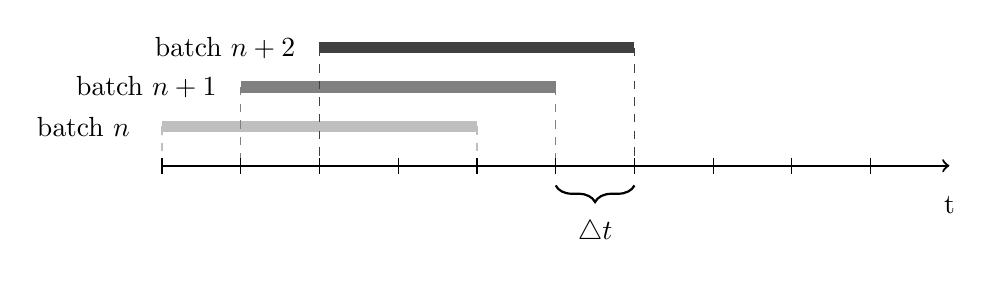
\begin{tikzpicture}[scale=1]

        \draw[lightgray, line width=4pt] (0,.5) -- (4,.5);
        \draw[lightgray, dashed] (0,.5) -- (0,0);
        \draw[lightgray, dashed] (4,.5) -- (4,0);
        \node[align=right] at (-1,.5) {batch $n$};

        \draw[gray, line width=4pt] (1,1) -- (5,1);
        \draw[gray, dashed] (1,1) -- (1,0);
        \draw[gray, dashed] (5,1) -- (5,0);
        \node[align=right] at (-.2,1) {batch $n + 1$};

        \draw[darkgray, line width=4pt] (2,1.5) -- (6,1.5);
        \draw[darkgray, dashed] (2,1.5) -- (2,0);
        \draw[darkgray, dashed] (6,1.5) -- (6,0);
        \node[align=right] at (0.8,1.5) {batch $n + 2$};

        \node[align=center] at (5.5,-0.85) {$\triangle t$};
        \node[align=center] at (10,-0.5) {t};

        \draw [thick,->] (0,0) -- (10,0);
        \foreach \x in {0,...,9} \draw (\x,0.1) -- (\x,-0.1);

        \draw [thick,decorate,decoration={brace,amplitude=6pt,raise=0pt,mirror}] (5,-0.25) -- (6,-0.25);

        \end{tikzpicture}

    \caption{Timeline showing the sliding window approach}
    \label{fig:timeline}
\end{figure}

\paragraph{Finding pairs clusters}
Thus we define our two events as follows:
To be able to compare clusters of different batches with each other, we have to find pairs of clusters between batches, which describe the same story. This is done by applying the same assumptions as for the scoring function used in the evaluation. Therefore clusters are paired based on their similarity calculated with the Jaccard index as shown in equation \ref{equ:similarity}. If the similarity is above a certain threshold, both clusters are seen as describing the same story.

\paragraph{Sliding window}

An important consideration for determining existing or new clusters is the overlap of samples between batches. If the overlap is too small, similar clusters will no longer be detected as such, which would result in an increasingly high error rate. Finding optimal values for the step size between batches and the number of samples for each batch is therefore essential for our online clustering approach.

\subsubsection{Implementation}
\label{sec:online_clustering_implementation}

The online clustering implemented for this thesis does not operate in a true online setting, but rather it takes our existing test data and simulates a data stream over time. The simulated approach allows us to directly compare the resulting events with the ground truth and thus evaluate different settings. The implementation is done with Python and runs in a similar dockerized environment as the evaluation framework.

\paragraph{Comparing clusters}
To detect events between batches of clusterings,
we have find pairs of clusters describing the same story.
This problem is solved in the evaluation framework as part of the scoring function,
by calculating the similarity for each possible cluster pair.
The resulting time complexity is $O(n^2)$, which we deemed acceptable for the static evaluation.
However in a dynamic setting such as the online clustering, performance is an important factor,
since it restricts the lengths of the time delta between batches and the overall batch size.
Thus we decided to use Locality-Sensitive Hashing (LSH)\cite{alex2015practical} to find similar clusters.
This reduces the time complexity to $O(log(n))$.
The implementation for LSH is provided by the datasketch library\cite{eric_zhu_2017_290602}.

% TODO explain LSH?

\paragraph{Detecting Events}
Once we have found pairs of clusters, which represent the same story, detecting events becomes trivial.
For each pair we look for news articles, which are only present in the new cluster.
These articles are then summarized in as an extension of an existing event.
Clusters from the new batch without a matching cluster from the previous batch
are seen as new events.

\paragraph{Measuring the quality of events} 
Since events are themselves clusters of news articles, we apply the MP-Score to measure detected events against events taken from the ground truth. This gives an indication if the detected events contain the same news articles as true events and thus the rate of false positives and false negatives. Calculating the score is $O(n^2)$, but since the application runs on a simulated timeline, time complexity is only a minor concern. 

\paragraph{CLI} The application provides a command line interface to run the simulation with different parameters such as the start date, number of days to run and the batch size.

\begin{lstlisting}[caption=Command line interface for the online clustering, label={lst:cli_online_clustering}]
    usage: online_clustering.py [-h] [--full-cluster] [--verbose] [--rows ROWS]
                            [--full_rows FULL_ROWS] --date DATE
                            [--run_n_days RUN_N_DAYS] [--threshold THRESHOLD]

Run the batchwise clustering over a simulated stream of news articles.

required arguments:
  --date DATE           

optional arguments:
  -h, --help            show this help message and exit
  --full-cluster        run a full clustering once a day
                        default: False
  --verbose             
                        default: False
  --rows ROWS           number of samples to process per batch
                        default: 1000
  --full_rows FULL_ROWS
                        number of samples to process for the full clustering
  --run_n_days RUN_N_DAYS
                        number of days to run the batchwise clustering
                        default: 1
  --threshold THRESHOLD
                        similarity threshold for cluster matching
                        default: 0.75

\end{lstlisting}

% TODO clarify event vs topic vs story and be consistent with the usages!

\section{Results}

\subsection{Clustering Evaluation}

The goal of this evaluation is to measure the accuracy of HDBSCAN, with different parameters and preprocessing methods. The most suitable approach will then be used for the online clustering to detect changes in a news stream.

\subsubsection{Setup}

\paragraph{Text Preprocessing}

 The first step in working with text is to apply Natural Language Processing techniques for improving the quality of the data before clustering it. We look the five different preprocessing methods  as described in section \ref{} and evaluate each. The methods are:
 \begin{itemize}
     \item Full text with stop word removal
     \item Keyterms
     \item Named Entities
     \item Lemmatization
     \item Stemmatization
 \end{itemize} 

\paragraph{Text Vectorization} Before the text can be clustered, it has to be transformed into a vector space model. We look at two different models:
\begin{itemize}
    \item Word Frequency
    \item tf-idf
\end{itemize}

\paragraph{Parameters} HDBSCAN has a range of parameters, which can be tuned to fit our dataset. We focus on the two primary ones:
\begin{itemize}
    \item Min cluster size: The minimum size of a cluster. We run the evaluation with a range from two to nine as the $min\_cluster\_size$. 
    \item Metric: The distance measure between points. We apply the metrics "cosine" and "euclidean". 
    
\end{itemize}

The primary parameter for K-Means is the number of clusters. Since K-Means is used as a baseline to evaluate HDBSCAN, we provide the true number of clusters for each run. Therefore K-Means runs with an optimal starting point. 

\paragraph{Running the evaluation} The evaluation is done with different sets of news articles per run. This means if we define a run to use 30 stories and set it to repeat five times, each repeat will load 30 different stories from the dataset. This is done to get a more diverse set of samples. Each run will be repeated at least three times. Lower numbers of stories allow for more repetitions due to lower processing times.   

\subsubsection{Evaluation}

The first run is done with 60 stories, which results in approximately 2000 news articles, over five repetitions. Table \ref{tab:cluster_parameters} shows the resulting accuracy for each parameter in combination with each preprocessing method and vector space model. The highest score per parameter is highlighted as bold. The first insight we get is the variety in accuracy scores for different min cluster sizes. The lowest min cluster size results in the lowest accuracy, while increasing this parameter leads to an increasingly better score. The highest accuracy is reached with a min cluster size of six, while increasing it further reduces the score again. The large difference in accuracies between different min cluster sizes, shows the importance this parameters has on the quality of the clustering and requires some knowledge of the data beforehand. In our case we have a wide range of different cluster sizes as shown in Figure \ref{fig:articles_per_story_distribution}, with clusters containing as little as two news articles. Based on this distribution we expected the min size cluster size to be low. The distribution also explains the drop in accuracy after a min cluster size of 6, since an increasingly number of clusters are being ignored.

\begin{table}[h]
    \centering
    \scalebox{0.65}{
    \begin{tabular}{|l|rrrrr|rrrrr|}
        \hline
        \textbf{Clustering} & \multicolumn{5}{ |c| }{\textbf{Word Frequency}} & \multicolumn{5}{ |c| }{\textbf{tf-idf}} \\
        \hline
        \textbf{HDBSCAN} & Full Text &  Keyterms & Entities & Lemmatized & Stemmed & Full Text &  Keyterms & Entities & Lemmatized & Stemmed \\
        \hline
        min\_size: 2, metric: cosine    & 0.289 & 0.265 & 0.223 & \textbf{0.305} & 0.297 & 0.286     & 0.268 & 0.26      & 0.296     & 0.3       \\
        min\_size: 2, metric: euclidean & 0.101 & 0.093 & 0.110 & 0.101     & 0.106 & 0.301     & 0.170 & 0.241     & \textbf{0.306} & 0.301     \\
        min\_size: 3, metric: cosine    & 0.488 & 0.456 & 0.465 & 0.48      & 0.487 & 0.472     & 0.446 & 0.457     & \textbf{0.493} & 0.478     \\
        min\_size: 3, metric: euclidean & 0.172 & 0.129 & 0.176 & 0.174     & 0.182 & 0.472     & 0.306 & 0.464     & \textbf{0.500} & 0.478     \\
        min\_size: 4, metric: cosine    & 0.630 & 0.555 & 0.625 & 0.552     & 0.577 & 0.577     & 0.586 & \textbf{0.646} & 0.589     & 0.581     \\
        min\_size: 4, metric: euclidean & 0.320 & 0.182 & 0.214 & 0.315     & 0.332 & 0.611     & 0.416 & 0.559     & 0.613     & \textbf{0.615} \\
        min\_size: 5, metric: cosine    & 0.716 & 0.652 & 0.656 & \textbf{0.718} & 0.718 & 0.688     & 0.664 & 0.632     & 0.686     & 0.692     \\
        min\_size: 5, metric: euclidean & 0.355 & 0.217 & 0.266 & 0.41      & 0.389 & \textbf{0.703} & 0.512 & 0.607     & 0.686     & 0.692     \\
        min\_size: 6, metric: cosine    & 0.693 & 0.715 & 0.608 & 0.701     & 0.708 & 0.738     & 0.729 & 0.613     & \textbf{0.751} & 0.747     \\
        min\_size: 6, metric: euclidean & 0.179 & 0.280 & 0.292 & 0.202     & 0.164 & 0.738     & 0.408 & 0.622     & \textbf{0.778} & 0.763     \\
        min\_size: 7, metric: cosine    & 0.631 & 0.611 & 0.552 & 0.643     & 0.634 & 0.689     & 0.685 & 0.553     & 0.718     & \textbf{0.722} \\
        min\_size: 7, metric: euclidean & 0.122 & 0.392 & 0.307 & 0.073     & 0.099 & 0.689     & 0.336 & 0.539     & 0.718     & \textbf{0.722} \\
        min\_size: 8, metric: cosine    & 0.571 & 0.603 & 0.514 & 0.592     & 0.574 & 0.685     & 0.647 & 0.531     & \textbf{0.711} & 0.695     \\
        min\_size: 8, metric: euclidean & 0.056 & 0.339 & 0.338 & 0.025     & 0.057 & 0.685     & 0.286 & 0.522     & \textbf{0.711} & 0.695     \\
        min\_size: 9, metric: cosine    & 0.542 & 0.569 & 0.476 & 0.544     & 0.541 & 0.602     & 0.614 & 0.499     & 0.637     & \textbf{0.640} \\
        min\_size: 9, metric: euclidean & 0.065 & 0.236 & 0.310 & 0.025     & 0.033 & 0.602     & 0.216 & 0.475     & 0.637     & \textbf{0.640} \\
        \hline
        \textbf{K-Means} & \multicolumn{5}{ |c| }{}  & \multicolumn{5}{ |c| }{} \\
        \hline
        n\_cluster: n\_true              & 0.531 & 0.588 & 0.514 & 0.536     & 0.536 & \textbf{0.713} & 0.653 & 0.584     & 0.672     & 0.693     \\
        \hline
    
    \end{tabular}   
    }
    \caption{Accuracy for combinations of parameter and preprocessing with a sample size of 60 stories (approx. 2000 articles)}
    \label{tab:cluster_parameters}
\end{table}

Comparing the two vector models, shows the majority of best scores per parameter achieved by tf-idf. Additionally the different metrics show a significant difference when using the vector model based on word count. With tf-idf the difference between both metrics is often negligible.

As for the optimal preprocessing, lemmatization appears to provide the highest accuracy in general or at least being fairly close to the highest score. This is to be expected, since lemmatization reduces the dimensions by grouping words into their base form, while still retaining most of the text. In contrast to keyterm and entity extraction, which both result in a drastic reduction of the dimensions, and therefore less detail. It is important to note, that we used pretrained models for keyterm and entity extraction. Specifically training on a news corpus might improve the performance of both methods, but it was decided as to be out of scope for this thesis.

\begin{figure}[h]
    \centering
    \includegraphics[width=1\textwidth]{articles_per_story_distribution}
    \caption{Distribution of cluster sizes.}
    \label{fig:articles_per_story_distribution}
\end{figure}

After determining the optimal settings for text preprocessing and vectorization, we increase the sample sizes for our evaluation runs, to get a deeper insight into the behaviour of HDBSCAN with larger datasets. Figure \ref{fig:hdbscan_parameters} shows the scores achieved with different parameters over an increasingly large set of samples. Based on this Figure we see the metric $cosine$ to be generally better than $euclidean$, even if $euclidean$ is occasionally more accurate.

TODO explain why cosine is generally better than euclidean
TODO explain min cluster sizes, but run with lemmatization

\begin{figure}[h]
    \centering
    \includegraphics[width=1\textwidth]{hdbscan_parameters}
    \caption{Accuracies for different parameters}
    \label{fig:hdbscan_parameters}
\end{figure}

One of the advantages HDBSCAN has over other clustering algorithms, is the ability to work with noise, since we intent on applying it in an online setting, where noisy data is to be expected. At the same time, the number of articles classified as noise should be kept to a minimum. However the noise ratio shown in Figure \ref{fig:noise_ratio_samples} is higher, than we would expect it to be based on our test data. A variety of factors play into the high noise ratio. One major influence is due to the used $min\_cluster\_size$. Each news article belonging to a cluster ignored due to a size too small, will be counted as noise. In addition to the false positives due to the min cluster size, the test data does still contain noisy data, even after our efforts in cleaning up the data as good as possible. Nonetheless the expected noise ratio based on the test data is less than 10\%, nowhere close to the 20\% of the current evaluation. Decreasing the noise ratio is certainly an important part in future improvements.

TODO calculate expected noise ratio based our min cluster sizes.

% experiment with min_samples

\begin{figure}[h]
    \centering
    \includegraphics[width=0.5\textwidth]{noise_ratio_samples}
    \caption{Number of news articles classified as noise.}
    \label{fig:noise_ratio_samples}
\end{figure}


Having found the optimal settings to run HDBSCAN with, we can start comparing the overall performance with K-Means. Figure \ref{fig:accuracy_kmeans_hdbscan} shows  a similar behaviour for both clustering methods in value and variance of the accuracy. Although HDBSCAN is generally more accurate than K-Means, the difference gets smaller with an increase in the sample size. 

Increasing the sample size results for both HDBSCAN and K-means in a small loss regarding the accuracy as can be seen in Figure \ref{fig:accuracy_kmeans_hdbscan}. However the accuracy seems to stabilize around the 0.7 mark.

\begin{figure}[h]
    \centering
    \includegraphics[width=0.5\textwidth]{accuracy_kmeans_hdbscan}
    \caption{Comparison of the average accuracy between K-means and HDBSCAN}
    \label{fig:accuracy_kmeans_hdbscan}
\end{figure}

While HDBSCAN and K-means provide a similar accuracy, the biggest difference can be noted in the processing time in relation to the number of samples. K-means has a time complexity of $O(n^2)$ in contrast to HDBSCAN with a time complexity of $O(nlog(n))$, which is demonstrated by Figure \ref{fig:processing_time_kmeans_hdbscan}. Although running the evaluation has also shown the space complexity for HDBSCAN to be substantially higher for larger amounts of samples than with K-means. Trying to run HDBSCAN with 100'000 news articles caused in a memory error, even with 64GB of RAM, while K-means was able to complete the clustering.

% TODO measure memory?

\begin{figure}[h]
    \centering
    \includegraphics[width=0.5\textwidth]{processing_time_kmeans_hdbscan}
    \caption{Processing time in seconds }
    \label{fig:processing_time_kmeans_hdbscan}
\end{figure}

Figure \ref{fig:cluster_difference_samples} shows, that the difference between predicted over the true number of clusters is fairly low and appears to be roughly linear with the overall number of clusters.  

\begin{figure}[h]
    \centering
    \includegraphics[width=0.5\textwidth]{cluster_difference_samples}
    \caption{Ratio of difference over predicted with true number of clusters}
    \label{fig:cluster_difference_samples}
\end{figure}

As a final note, we compare HDBSCAN with six different clustering methods taken from scikit-learn. Each method is run with a variety of parameters and the best scores are shown in Figure \ref{fig:different_clusterings}. HDBSCAN provides the highest accuracy, while being still being one of the fastest algorithms. Based on this data, we can assume HDBSCAN to be a good candidate for our use case.

\begin{figure}[h]
    \centering
    \includegraphics[width=0.5\textwidth]{different_clusterings}
    \caption{Comparison of different clustering methods with a sample size of approximately 1000 news articles}
    \label{fig:different_clusterings}
\end{figure}

\subsubsection{Conclusion}

% TODO: This conclusion belongs to the chapter "Conclusion"
The evaluation has shown HDBSCAN to be a good candidate to use for news clustering. It provides an better accuracy than K-means, while being significantly faster to process. The predicted number of clusters is consistent with an increasing number of samples and fairly close the truth. Additionally we have shown the required preprocessing and vectorization steps with the ideal parameters to achieve the most accurate results for our dataset. On the flip side the noise ratio is quite high and the space complexity is problematic with larger datasets. Overall HDBSCAN provides an acceptable accuracy, while still leaving room for further improvements.

\subsection{Online clustering}

\subsubsection{Setup}

The online clustering is done on a simulated stream of news articles based on the same data set as used in the clustering evaluation. This allows for direct comparison between the detected events and the ground truth. The settings to run the clustering are as follows:

\begin{itemize}
    \item Text preprocessing: Lemmatization
    \item Vectorizer: tf-idf
    \item Clustering method: HDBSCAN
    \item Min cluster size: 5
    \item Distance metric: cosine
\end{itemize}

The clustering is run over 30 days with a total of 42'916 news articles. The distribution of news articles this time period is illustrated in Figure \ref{fig:news_articles_over_time}.

\begin{figure}[h]
    \centering
    \includegraphics[width=0.5\textwidth]{news_articles_over_time}
    \caption{Incoming news articles over 30 days}
    \label{fig:news_articles_over_time}
\end{figure}

\subsubsection{Evaluation}

TODO evaluate different thresholds

TODO evaluate different time deltas

TODO show example with a specific topic e.g. when it first is detected, incoming news articles etc.

\begin{figure}[h]
    \centering
    \includegraphics[width=1\textwidth]{event_detection_by_date}
    \caption{Comparison between detected and true events with batch size of 2000 samples}
    \label{fig:event_detection_by_date}
\end{figure}

\begin{figure}[h]
    \centering
    \includegraphics[width=0.5\textwidth]{event_detection_overlap}
    \caption{Plot work in progress}
    \label{fig:event_detection_overlap}
\end{figure}

% analyse overlap size
% show incoming news articles
% show deletion events on full clusterings
\section{Conclusion}

\subsection{Summary}

We started our work by searching for a suitable data set to create our clustering evaluations with. The primary requirement was, to have data points with their corresponding cluster labels. Having a labelled data set allows us to apply external measures and evaluate a resulting clutering against the ground truth. After selecting a few data set for closer inspection, we settled on the News Aggregator Dataset, which contains 422'937 labelled news articles, where a label describes the story the news article is about. Since the same story label applies to multiple news articles, we could use this as a cluster descriptor. Unfortunately the data set only contained headlines, which did not contain enough information for our approach. Therefore we collected the full text from each news article based on the provided source url. The content retrieval process turned out to generate a significant amount of noise, due to expired urls, paywalls, parsing errors or wrong redirects. To reduce the noise, we applied different cleansing techniques and ended up with approximately XXX usable news articles.

Once the data set was ready, we designed an evaluation framework to automatically run clustering methods with a variety of settings. The focus was to find a combination of text preprocessing methods, vector space model and parameters for the clustering method, which would provide the best clustering. Furthermore we developed a custom scoring function to measure the results of a clustering, since existing measures proved to be unintuitive and biased against certain results, such as the number of clusters. After having done many clustering evaluations based on our test data, we focused on analysing the collected data for our primary clustering method HDBSCAN and compared it to \textit{k}-means. The analyse gave valuable insight into the behaviour of HDBSCAN with different vector space models combined with different preprocessing methods and parameters. We noted the initial good performance and the decrease in the quality of the clustering the bigger the sample size got. However the amount of news articles proved to be substantial with up to 30\%. Possible explanations were explored, such as actual noisy data and different representations of articles belonging to the same cluster with tf-idf.

Having determined the optimal settings in the HDBSCAN evaluation, we applied them in a simulated online setting for event detection. The event detection was accomplished by running the clustering in batches over time. Events are detected by comparing a batch with its predecessor. If a batch contains clusters, which do not appear in the previous batch, than those clusters are considered as new events. If a cluster did exist in the previous batch, we look at the difference in assigned news articles and can therefore detect changes in existing event. The detection of events is measured against the ground truth. We explored different batch sizes and similarity thresholds for finding pairs of clusters between batches. Since finding pairs of clusters, requires a large enough overlap in identical news articles, the batch size has to account for this factor with regards to the volume of incoming news articles through the data stream. Additonally since events are represented as clusters, the sum of events can be regarded as a subclustering of the overall clustering. Although this makes the subclustering more sensitive to inaccuracies in the overall clustering, which explains the high error rate we observed in detecting new events. In conlcusion we found the error rate in detected events to be rather high for our approach and therefore not applicable in a real world scenario in its current state. 

\subsection{Future work}


How can this work be improved further?

Using a center point as label for the event.

Improve vector space model

using different text data 

\begin{itemize}
    \item Improving space complexity and noise ratio of HDBSCAN.
    \item Alternatively, use HDBSCAN as an approximation for the number of clusters and a different clustering algorithm
    for the actual creation of the clusters.
\end{itemize}


\subsection{Lessons learned}
% State the 3 biggest lessons learned.
% E.g. HDBSCAN is slightly better than sklearn but way faster.
Good data set -> noise rate


knowing your score



\section{Index}
\label{sec:7_index}

% 6.1 Literaturverzeichnis
\subsection{Bibliography}
\renewcommand*{\UrlFont}{\rmfamily}
\printbibliography[heading=none]

% 6.2 Glossar

% Remove glossary title.
\renewcommand{\glossarysection}[2][]{}

% Add glossary entries.
\newglossaryentry{Vectorizer}
{
    name=vectorizer,
    description={A vectorizer transform a text into a numeric vector}
}
\newglossaryentry{Clustering}
{
    name=clustering,
    description={The task of grouping a set of objects based on their similarity}
}
\newglossaryentry{Docker}
{
    name=docker,
    description={A tool to package the application with all its dependencies as a single deployable unit and run it on independently from the underlying host}
}
\newglossaryentry{Dockerized}
{
    name=dockerized,
    description={An application environment running as a single or a collection of docker containers}
}
\newglossaryentry{API}
{
    name=api,
    description={An application programming interface allowing access to data or features of an application}
}

% Print glossary.
% \glsaddall
\subsection{Glossary}
\printglossary[type=main]

% 6.6 Abkürzungsverzeichnis

% 6.3 Abbildungsverzeichnis

% Remove the list of figures title.
\makeatletter
\renewcommand\listoffigures{%
        \@starttoc{lof}%
}
\makeatother

% Print the list of figures.
\subsection{List of Figures}
\label{subsec:7c_list_of_figures}

\listoffigures

% 6.4 Tabellenverzeichnis

% Remove the list of tables title.
\makeatletter
\renewcommand\listoftables{%
        \@starttoc{lot}%
}
\makeatother

% Print the list of tables.
\subsection{List of Tables}
\label{subsec:7d_list_of_tables}

\listoftables

\input{7g_index}

\section{Appendix}

\subsection{Algorithm for Accuracy Selection}

\begin{lstlisting}[language=Python, caption=Select relevant accuracy values from a accuracy matrix., label={lst:select_max_values}]
    def select_max_values(self, accuracy_matrix):
        unique_indices = dict()
        row_index = 0
        nrows = len(accuracy_matrix)
        
        while row_index < nrows:
            ignore_indices = set()
            max_value_found = False
    
            while not max_value_found:
                max_value = 0
                column = 0
                for col_index, value in enumerate(accuracy_matrix[row_index]):
                    if value >= max_value and col_index not in ignore_indices:
                        max_value = value
                        column = col_index
    
                if (
                    max_value > 0
                    and column in unique_indices
                    and unique_indices[column]["row_index"] != row_index
                    and unique_indices[column]["max_value"] > 0
                ):
                    if unique_indices[column]["max_value"] < max_value:
                        # The column is already used, but we found a better 
                        # candidate. We use the new candidate and set the 
                        # cursor to the old one to find a new max value.
                        old_row_index = unique_indices[column]["row_index"]
                        unique_indices[column]["row_index"] = row_index
                        row_index = old_row_index
                        unique_indices[column]["max_value"] = max_value
                        max_value_found = True
                    else:
                        # The column is already used by a better candidate.
                        ignore_indices.add(column)
                else:
                    # If max_value is greater than 0, we store the value as a 
                    # new candidate. Otherwise either the row does not match 
                    # any other column or the max_value was low and got 
                    # overridden by previous tries and no other match is available. 
                    if max_value > 0:
                        # The column is free to use
                        unique_indices[column] = {
                            "row_index": row_index,
                            "max_value": max_value,
                        }
                    max_value_found = True
                    row_index += 1
        
        return unique_indices
\end{lstlisting}


\end{document}
